\documentclass[aspectratio=169]{beamer}
\usepackage[utf8]{inputenc}
\usepackage{bookman}
\usetheme{Dresden}
\usepackage{graphicx}
\usepackage{hyperref}
\usepackage{todonotes}

\title[03-EDA-PCB]{EDA: PCB Layout}
\author{MedTech Prototyping Skills (BME290L)}
\institute[Palmeri (Spring 2023)]{Mark L. Palmeri, M.D., Ph.D.}
\date{April 04, 2023}
\logo{
\includegraphics[width=0.1\textwidth]{BME-HorizontalLogo-Web-Blue.png}}

\begin{document}

\frame{\titlepage}

\section{PCB Revisions}

\begin{frame}{PCB Revisions}
    \begin{columns}
        \begin{column}{0.5\textwidth}
            Revising a PCB is inevitable... and you will need to do make a few
            changes based on some "bugs" I am responsible for. 
        \end{column}
        \begin{column}{0.5\textwidth}
            \centerline{
\includegraphics[width=1.0\textwidth]{changelog.png}}
        \end{column}
    \end{columns}
\end{frame}

\begin{frame}{Bug 1: Voltage Source}

    \begin{columns}
        \begin{column}{0.4\textwidth}
           \begin{itemize}
            \item 6 V source $\rightarrow$ 9 V
            \begin{itemize}
                \item \texttt{7805} dropout Voltage (min 2.5 V)
                \item \texttt{D101} threshold voltage
            \end{itemize}
            \item Reverse polarity LED $\rightarrow$ rectification diode
            \begin{itemize}
                \item Lower threshold voltage (not hard requirement)
                \item Higher max current
            \end{itemize}
           \end{itemize} 
        \end{column}
        \begin{column}{0.6\textwidth}
            \centerline{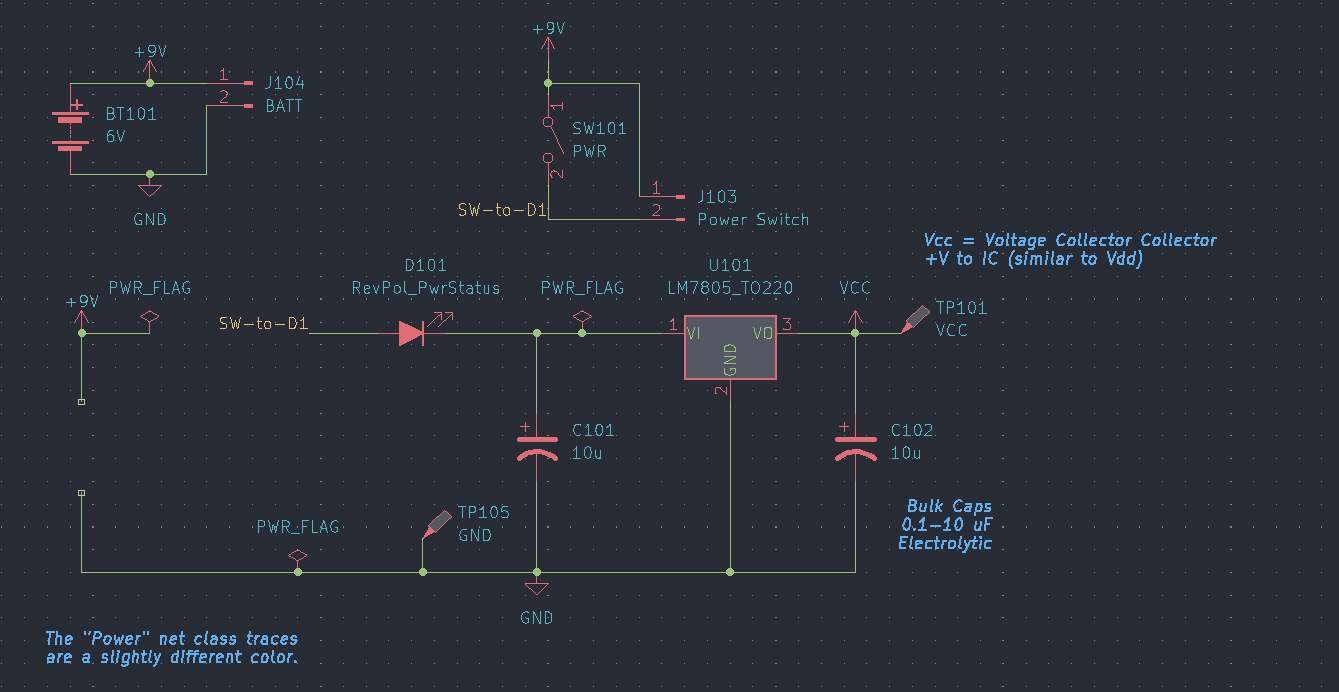
\includegraphics[width=1.0\textwidth]{pwr_ckt.png}}
        \end{column}
    \end{columns}

\end{frame}

\begin{frame}{Bug 2: Astable Oscillator Potentiometer}

    \centerline{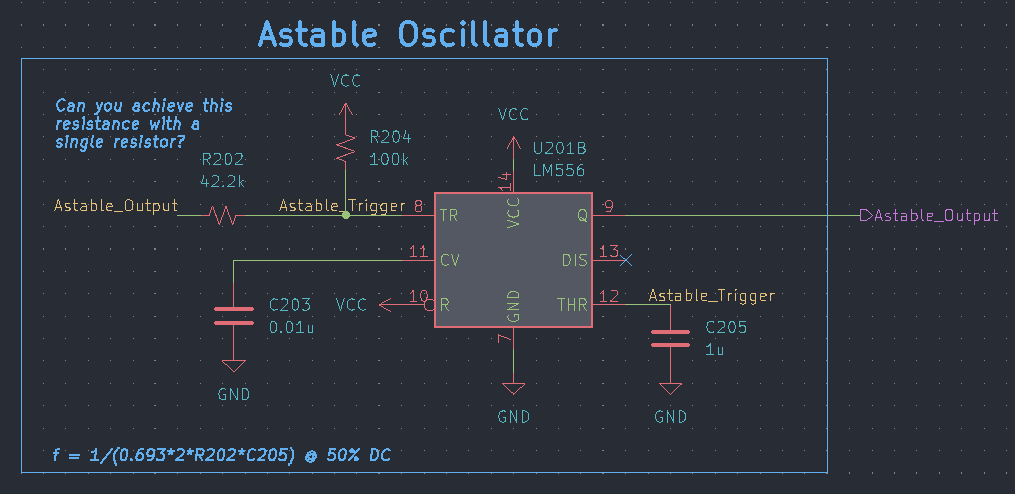
\includegraphics[width=0.7\textwidth]{astable_pot_fix.png}}

    \texttt{R202} was incorrectly labeled as \texttt{R204} in the astable
    frequency equation.  (Poor use of re-annotation tool.)

    \tiny{\url{https://www.electronics-tutorials.ws/waveforms/555_oscillator.html}}

\end{frame}

\section{Testing \& Debugging}

\begin{frame}{Connectivity Testing}
    \begin{columns}
        \begin{column}{0.5\textwidth}
        \begin{itemize}
            \item Done with the circuit \texttt{OFF} to make sure solder joints are good.
            \item Done to make sure things that shouldn't be connected aren't connected.
            \item Make sure no isolated ground islands.
        \end{itemize}
        \end{column}
        \begin{column}{0.5\textwidth}
            \centerline{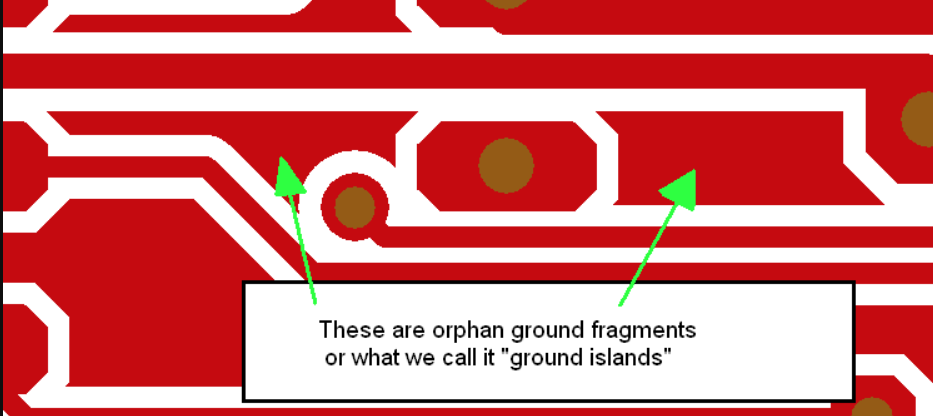
\includegraphics[width=1.0\textwidth]{ground_islands.png}}    
        \end{column}
    \end{columns}
\end{frame}

\begin{frame}{Voltage Source}
\begin{columns}
    \begin{column}{0.5\textwidth}
        \begin{enumerate}
            \item Test with all downstream ICs removed from sockets.  (Why?)
            \item Use power supply source (hijack switch header pin) and limit current (200 mA).
            \item Voltage before/after diode
            \item \texttt{7805} in/out voltages
            \item Min input voltage 7.5 V
            \item If output voltage $<$ 5 V, current draw too high (may occur when testing ICs).
        \end{enumerate}
    \end{column}
    \begin{column}{0.5\textwidth}
       \centerline{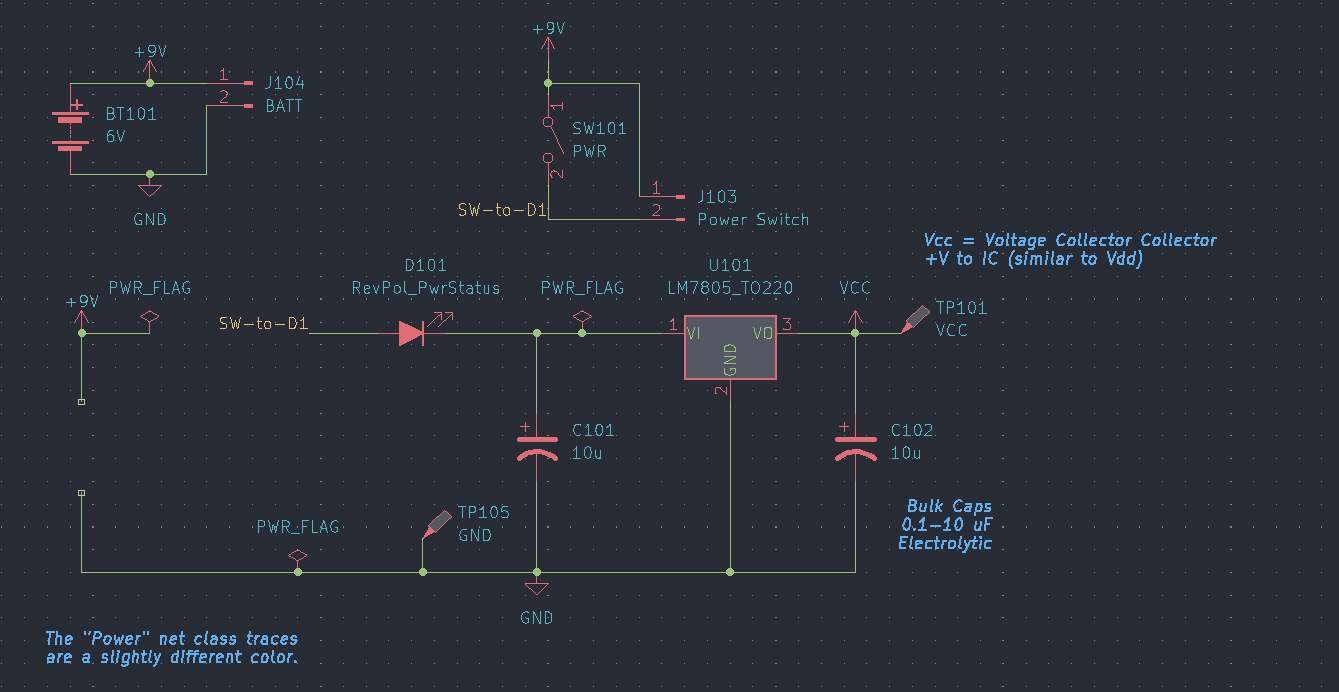
\includegraphics[width=1.0\textwidth]{pwr_ckt.png}} 
    \end{column}
\end{columns}
\end{frame}

\begin{frame}{Test Timers}

    \begin{columns}
        \begin{column}{0.5\textwidth}
            \begin{itemize}
                \item Test with only one timer on board at time.
                \item Power using voltage circuit.  Keep an eye on the current
                draw.
                \item You should have test points on the outputs of these timers
                that should facilitate testing with oscilloscope.
                \item Modulate potentiometer resistance and measure change in
                output.
            \end{itemize}
        \end{column}
        \begin{column}{0.5\textwidth}
            \centerline{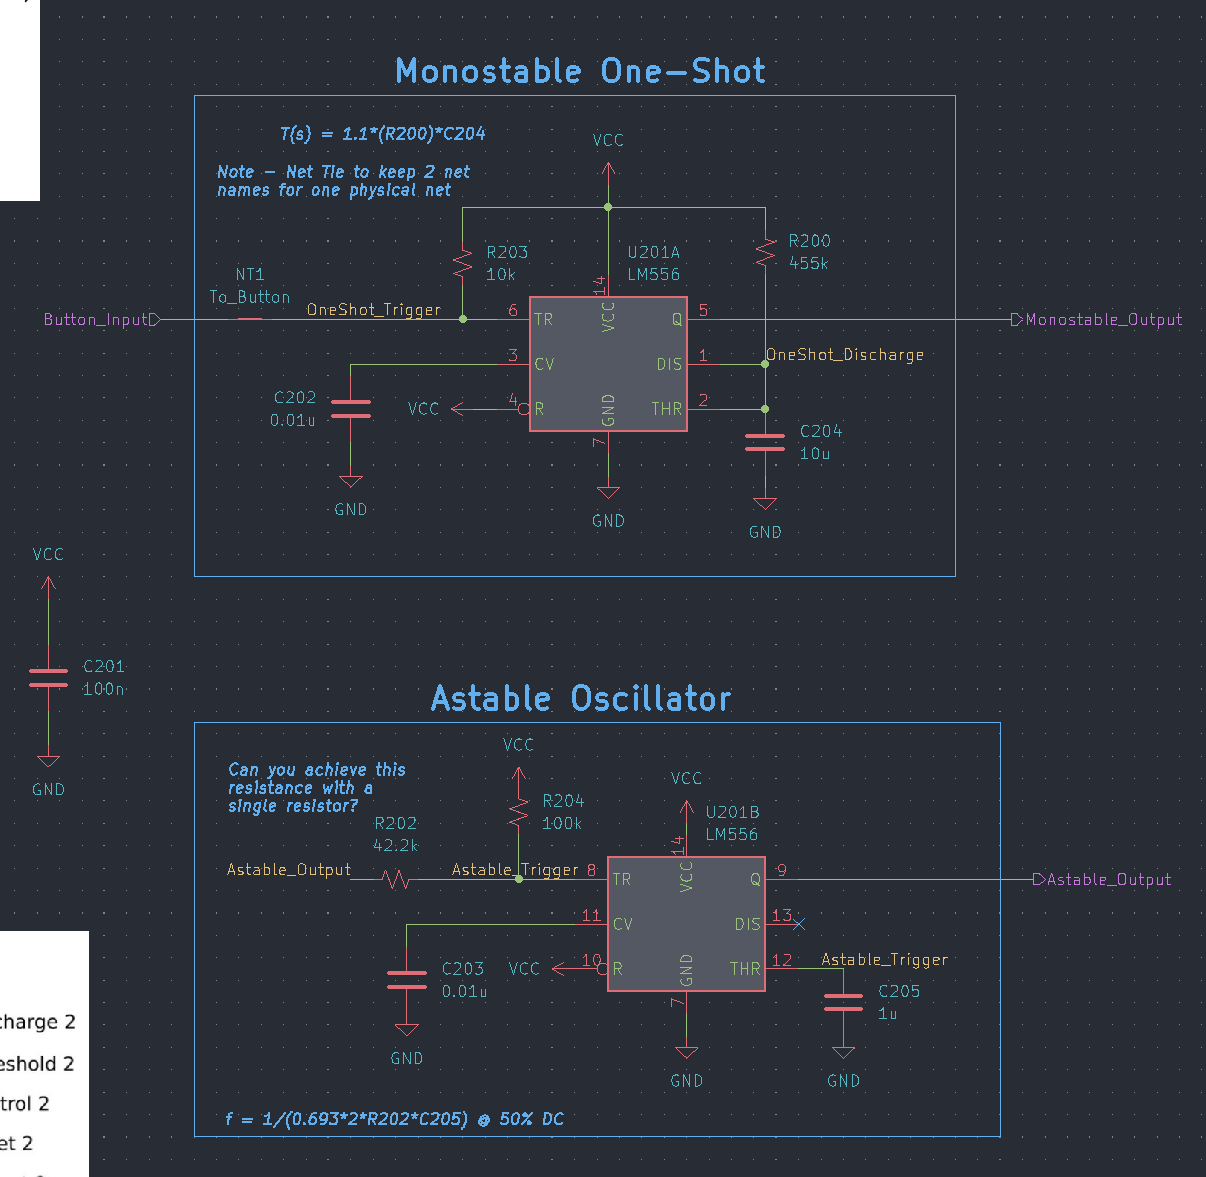
\includegraphics[width=0.8\textwidth]{schematic_timers.png}} 
        \end{column}
    \end{columns}

\end{frame}

\begin{frame}{Test Logic Gates}
    \begin{itemize}
        \item Power using voltage circuit.
        \item Remove timer IC.
        \item Manually set input logic states (0/5 V) and test output states
        using test points (do not connect the LEDs; why?).
        \item Graduate to test using timer outputs.
    \end{itemize}

\end{frame}

\begin{frame}{Test Points}
    \centerline{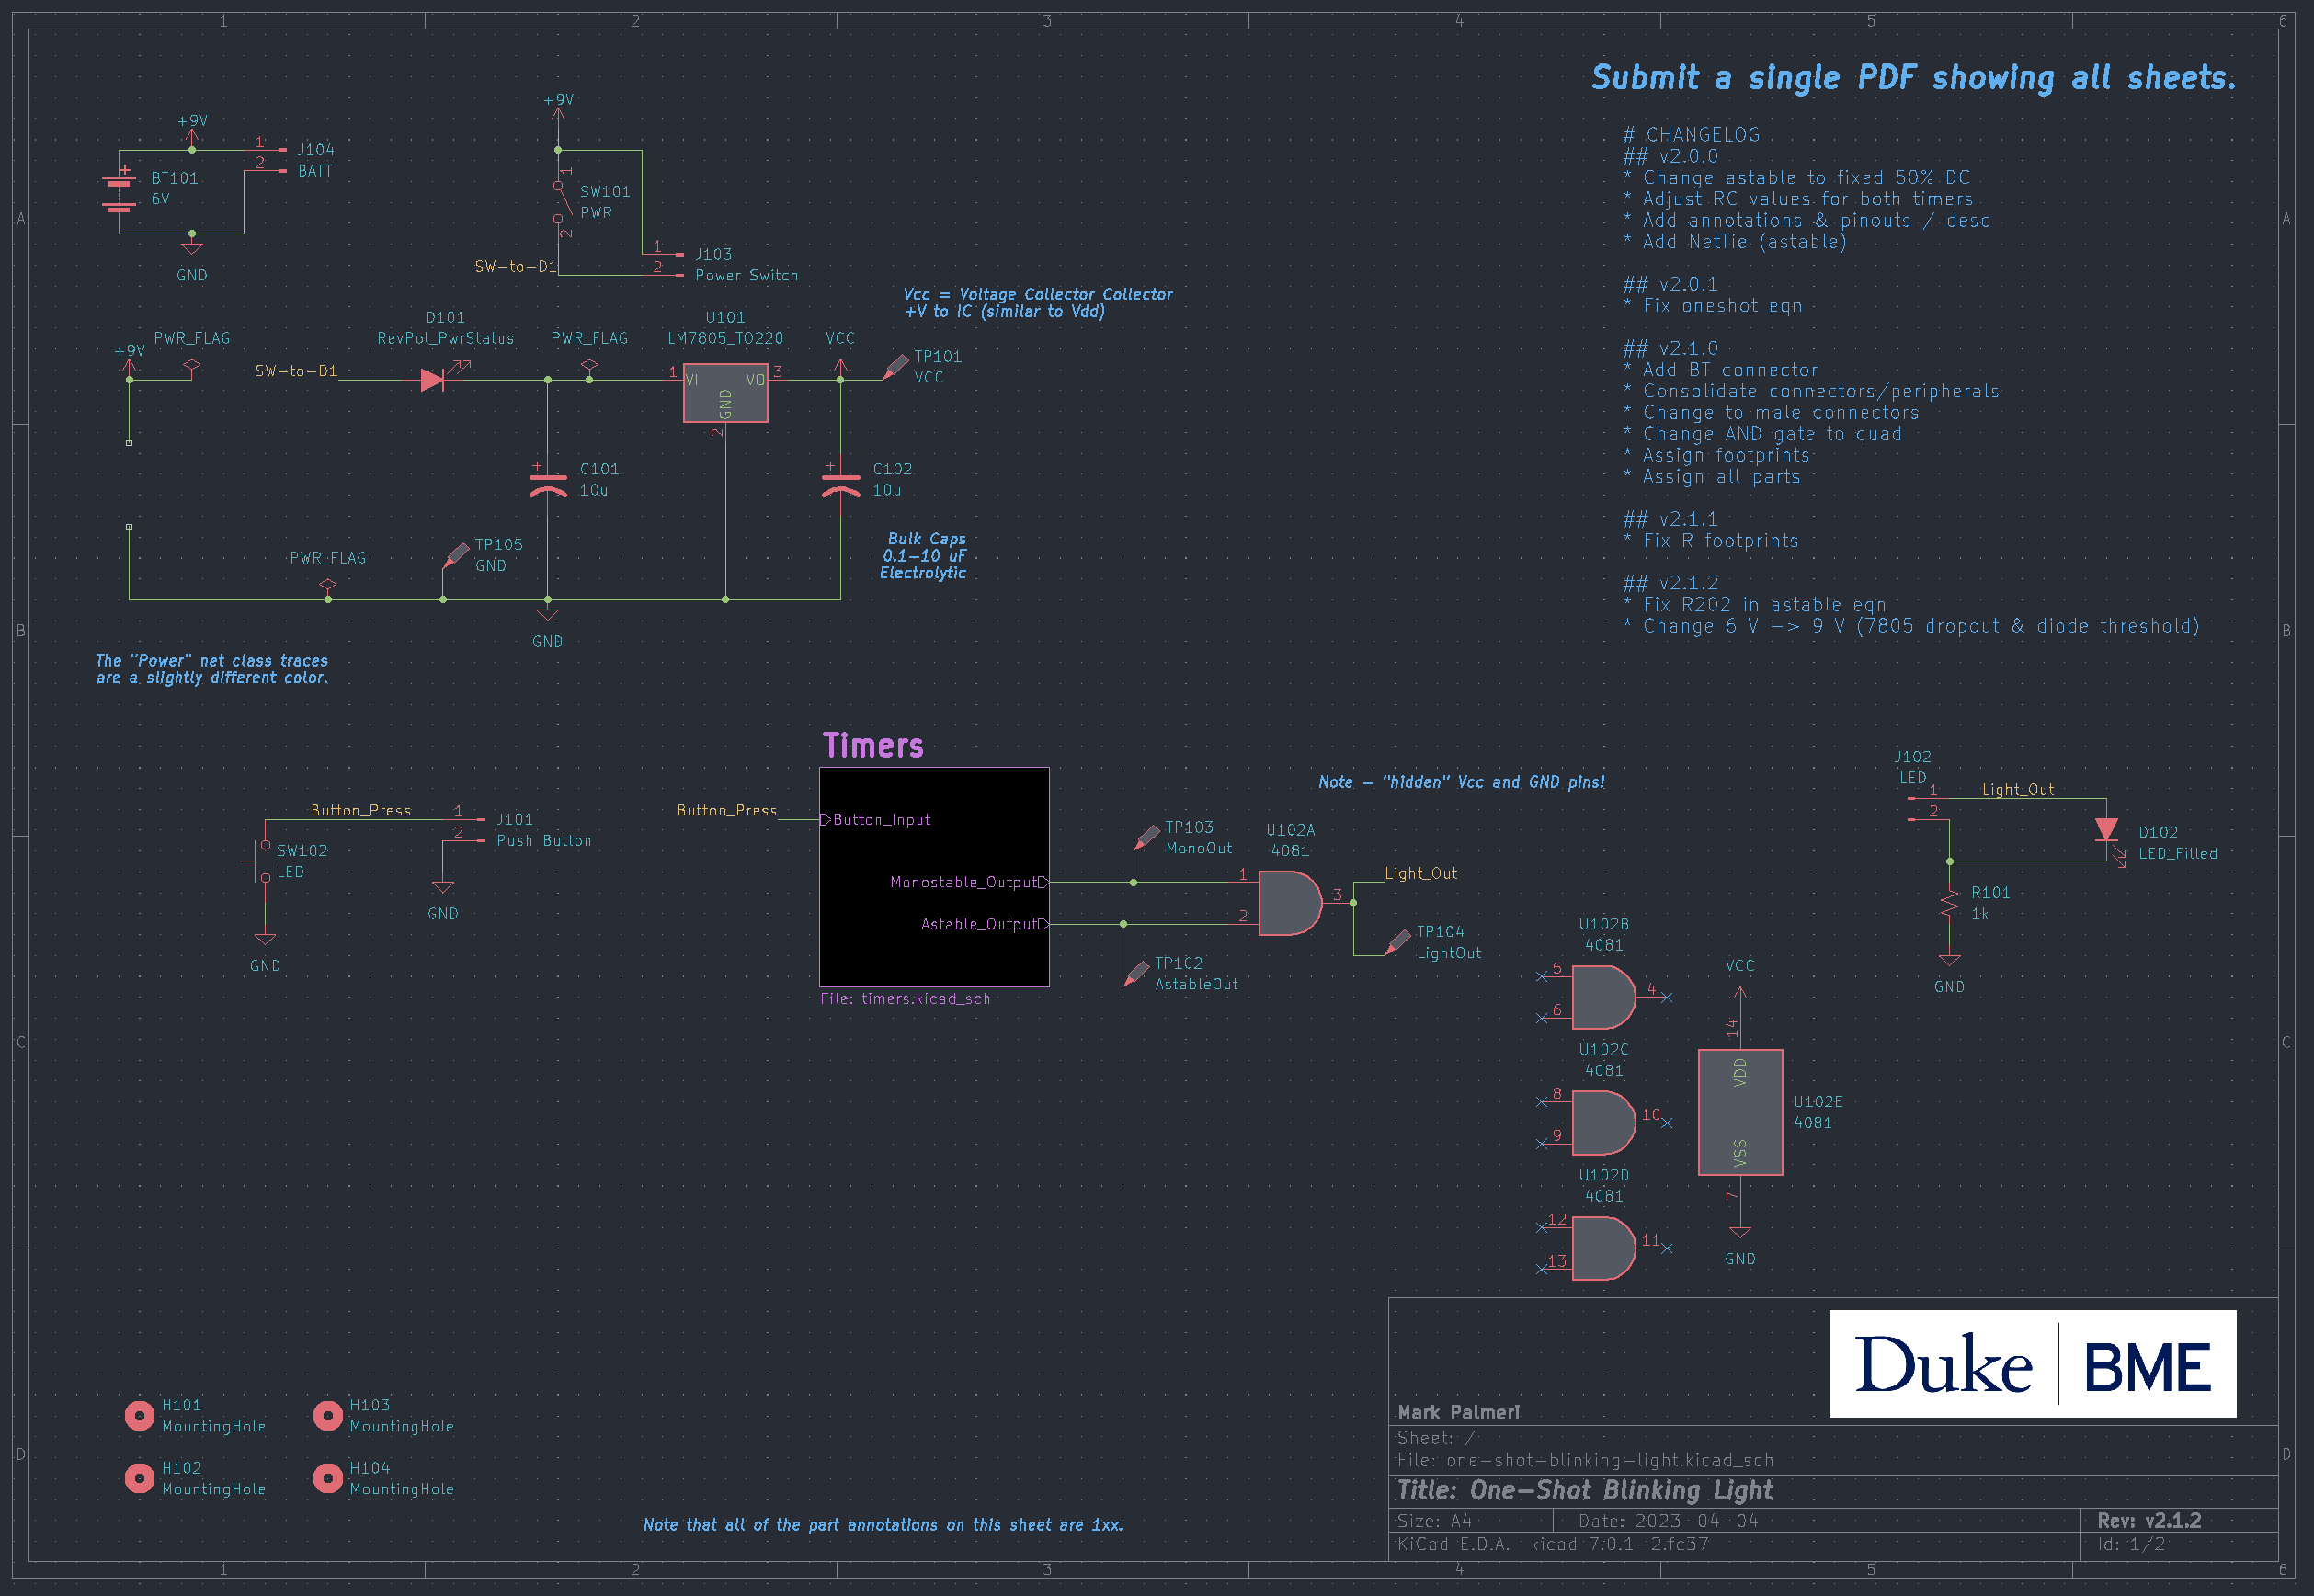
\includegraphics[width=0.6\textwidth]{schematic_root.png}}
\end{frame}

\begin{frame}{Test Everything}
\begin{itemize}
    \item Test the output LEDs with the circuit off, and manually applying 5 V to each.
    \item Confirm appropriate current draw.
    \item Put everything together and test!
\end{itemize}

\end{frame}

\begin{frame}{What if something doesn't work?}
\begin{itemize}
    \item By isolating each sub-circuit as much as possible, we are more focused on what might be wrong.
    \item Check circuit topology and connectivity.
    \item Check part validity / polarity.
    \item Check intermediate function (e.g., RC charge / discharge on timers).
\end{itemize}

\end{frame}

\section{ADALM2000 / Scopy}
\begin{frame}{ADALM2000}

    \begin{columns}
        \begin{column}{0.5\textwidth}
    We are short on some bench equipment, but we have some USB-based testing equipment to use!
            
        \end{column}
        \begin{column}{0.5\textwidth}
    \centerline{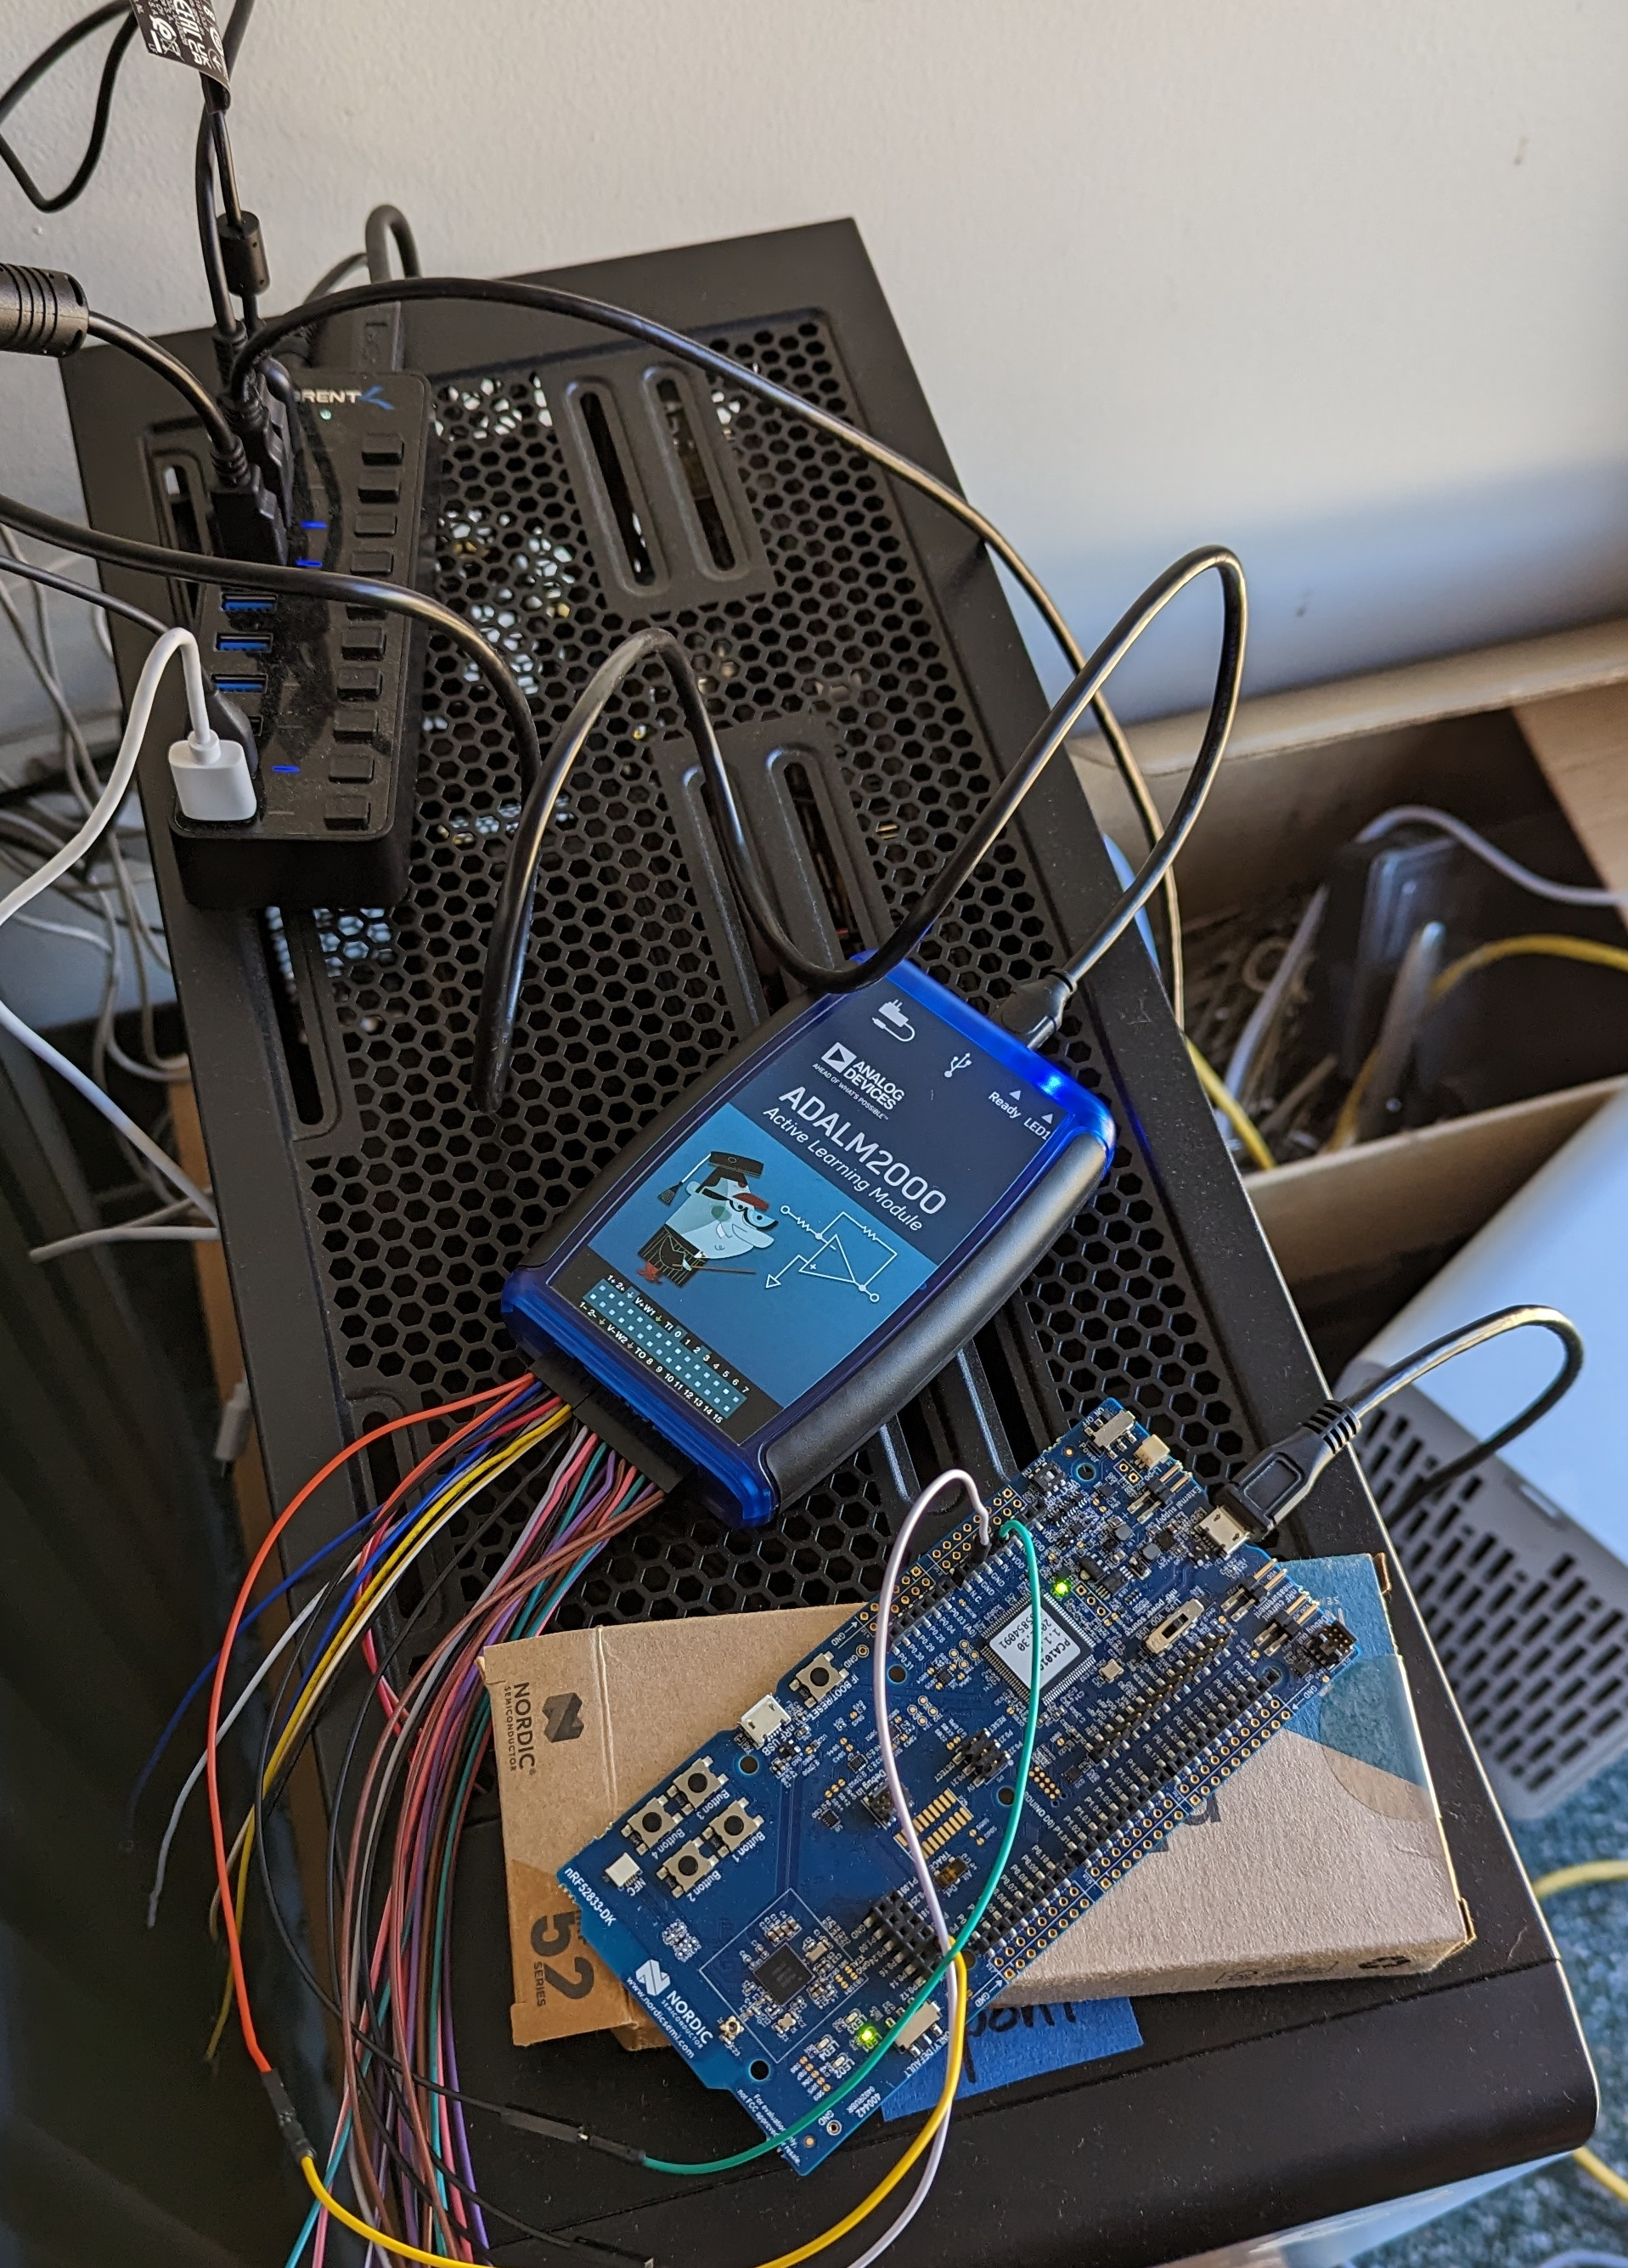
\includegraphics[width=0.5\textwidth]{adalm2000.jpg}}
            
        \end{column}
    \end{columns}



\end{frame}

\begin{frame}{Scopy}

    \begin{columns}
        \begin{column}{0.5\textwidth}
            \begin{itemize}
                \item You can use your laptop to provide (limited!!)
                voltage/current, act as a multimeter / oscilloscope.
                \item \url{https://wiki.analog.com/university/tools/m2k/scopy}
                \item \url{https://wiki.analog.com/university/tools/m2k/scopy/oscilloscope}
            \end{itemize}    
        \end{column}
        \begin{column}{0.5\textwidth}
            \centerline{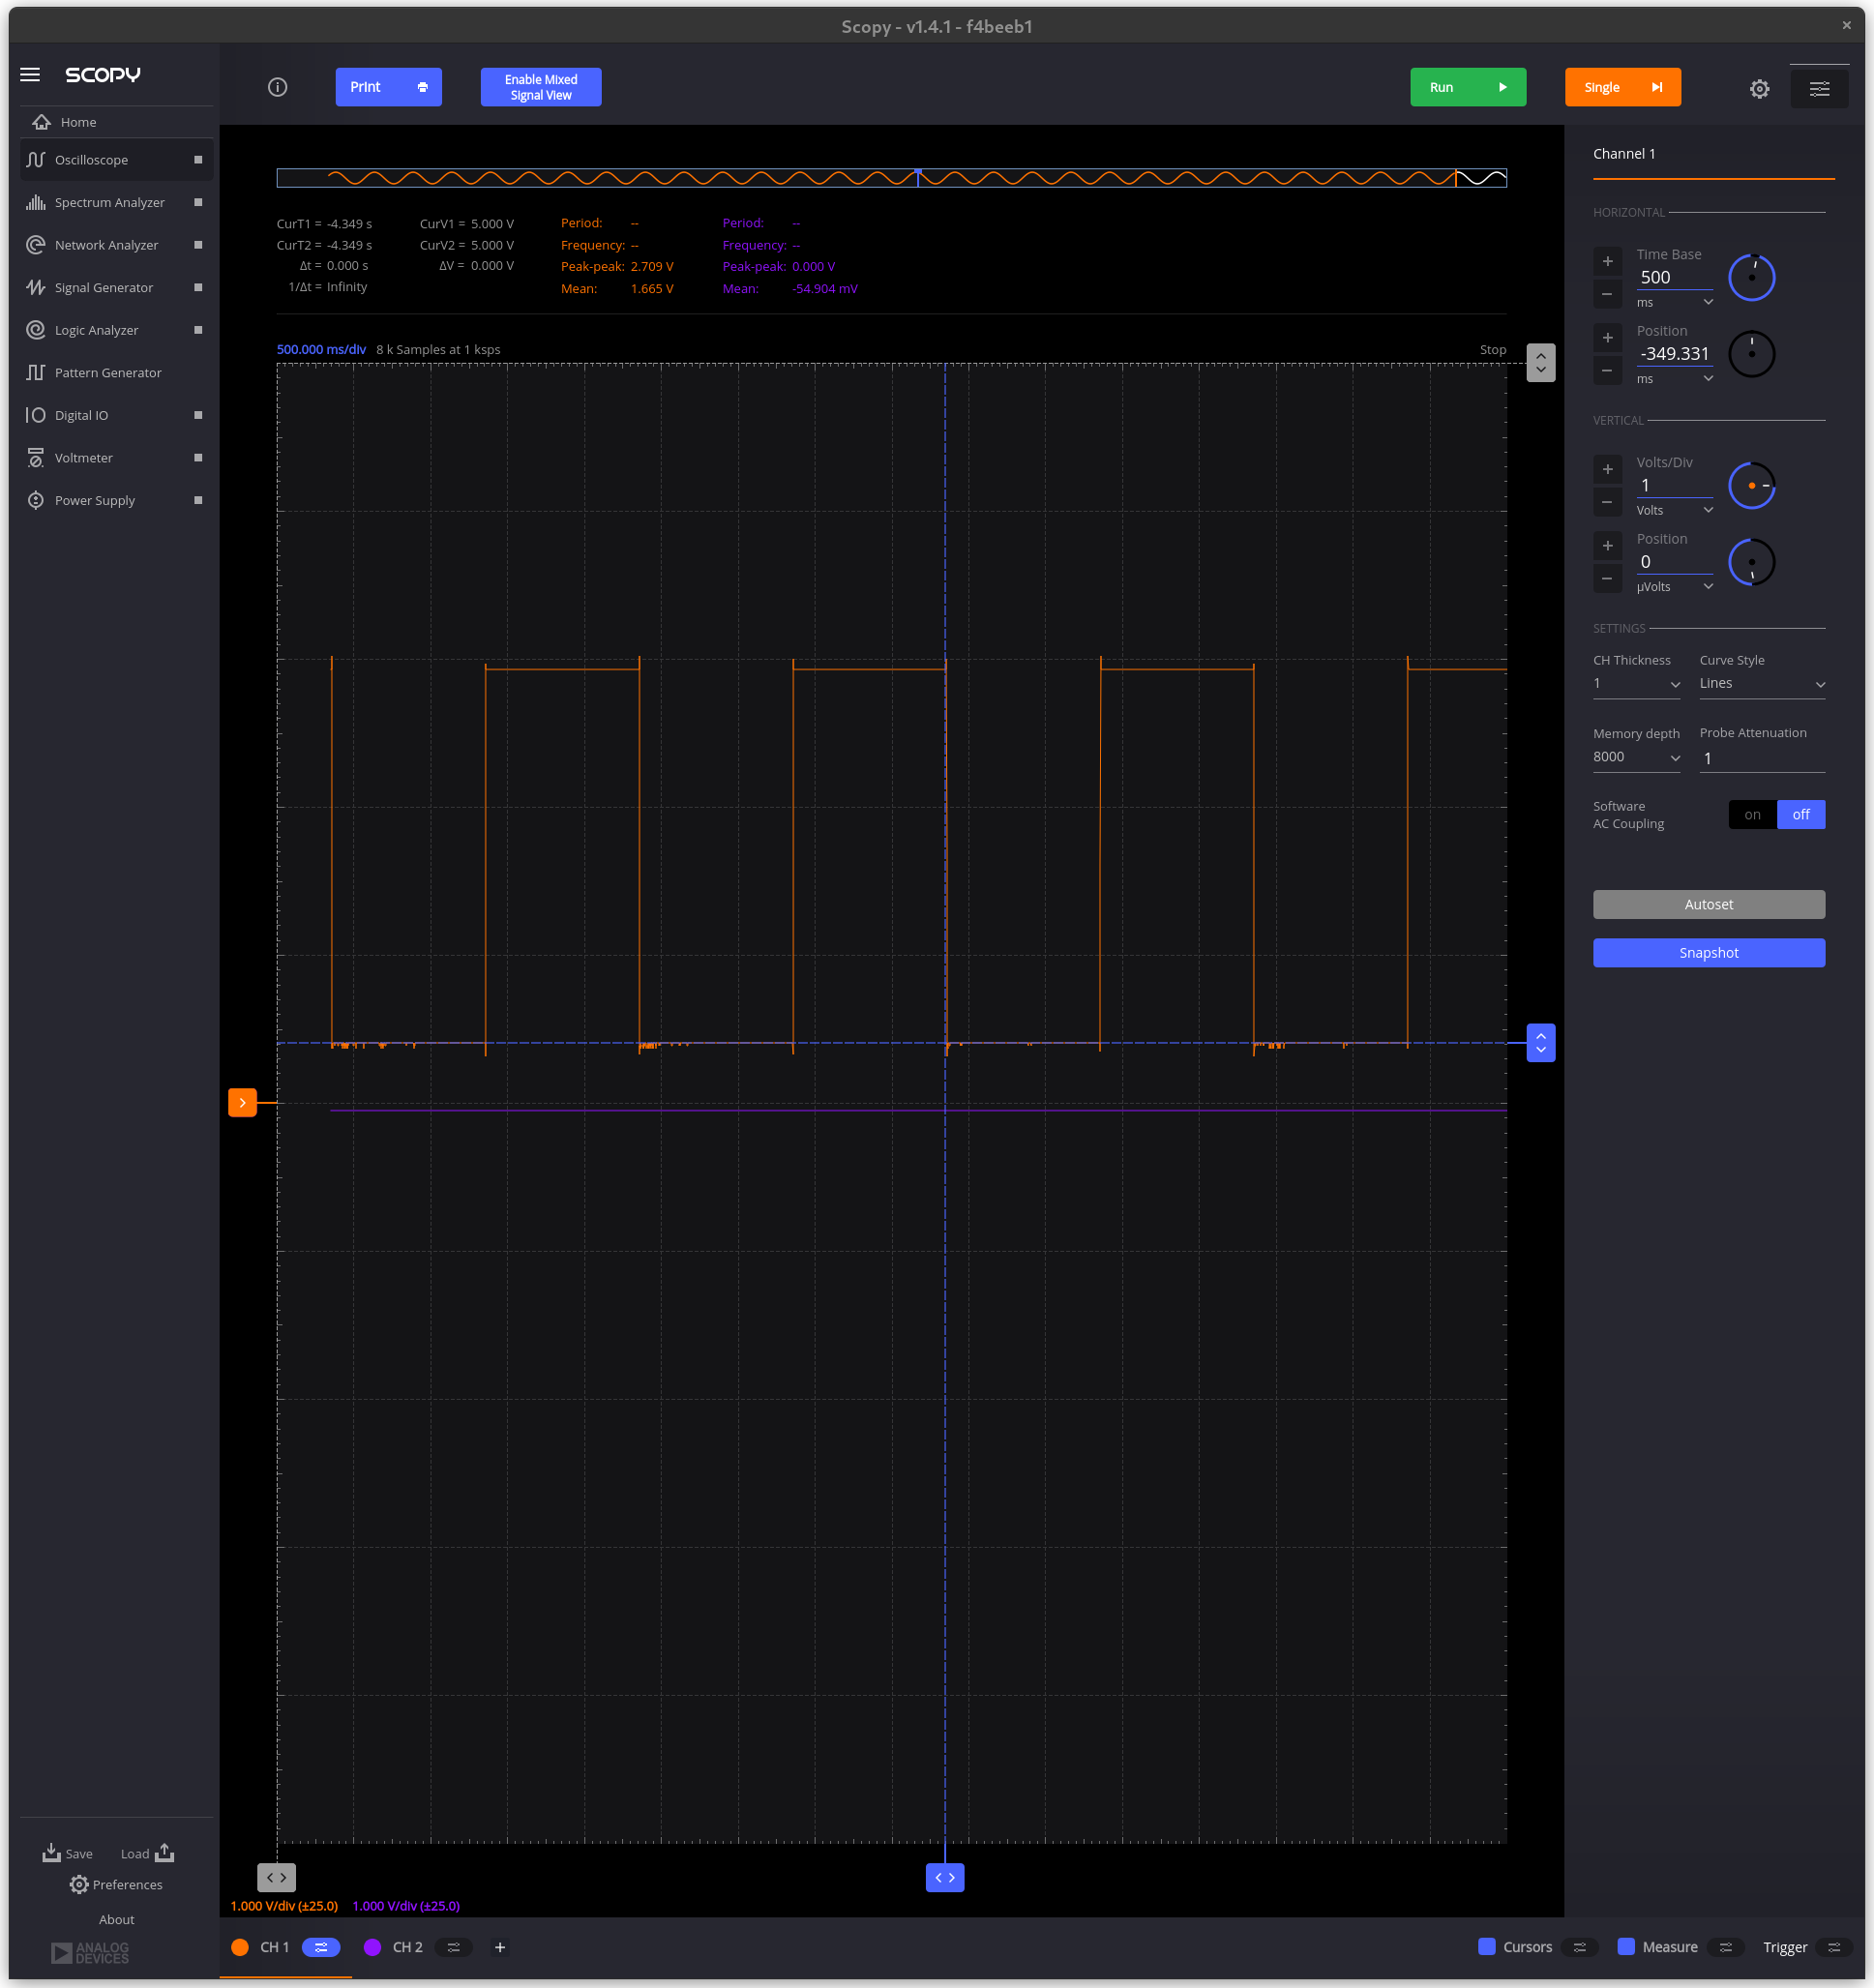
\includegraphics[width=0.75\textwidth]{scopy.png}}
        \end{column}
    \end{columns}

\end{frame}

\section{Resources}
\begin{frame}
  \frametitle{Resources}
  \begin{itemize}
    \item \href{https://www.electronics-tutorials.ws/waveforms/555_oscillator.html}{555 Oscillator Tutorial}
    \item \href{https://www.analog.com/en/design-center/evaluation-hardware-and-software/evaluation-boards-kits/adalm2000.html}{ADALM2000}
    \item \href{https://wiki.analog.com/university/tools/m2k/scopy}{Scopy: Installation}
    \item \href{https://wiki.analog.com/university/tools/m2k/scopy/oscilloscope}{Scopy: Oscilloscope}
  \end{itemize}
\end{frame}

\end{document}
